\documentclass{book}
\usepackage[a4paper,top=2.5cm,bottom=2.5cm,left=2.5cm,right=2.5cm]{geometry}
\usepackage{makeidx}
\usepackage{natbib}
\usepackage{graphicx}
\usepackage{multicol}
\usepackage{float}
\usepackage{listings}
\usepackage{color}
\usepackage{ifthen}
\usepackage[table]{xcolor}
\usepackage{textcomp}
\usepackage{alltt}
\usepackage{ifpdf}
\ifpdf
\usepackage[pdftex,
            pagebackref=true,
            colorlinks=true,
            linkcolor=blue,
            unicode
           ]{hyperref}
\else
\usepackage[ps2pdf,
            pagebackref=true,
            colorlinks=true,
            linkcolor=blue,
            unicode
           ]{hyperref}
\usepackage{pspicture}
\fi
\usepackage[utf8]{inputenc}
\usepackage{mathptmx}
\usepackage[scaled=.90]{helvet}
\usepackage{courier}
\usepackage{sectsty}
\usepackage{amssymb}
\usepackage[titles]{tocloft}
\usepackage{doxygen}
\lstset{language=C++,inputencoding=utf8,basicstyle=\footnotesize,breaklines=true,breakatwhitespace=true,tabsize=4,numbers=left }
\makeindex
\setcounter{tocdepth}{3}
\renewcommand{\footrulewidth}{0.4pt}
\renewcommand{\familydefault}{\sfdefault}
\hfuzz=15pt
\setlength{\emergencystretch}{15pt}
\hbadness=750
\tolerance=750
\begin{document}
\hypersetup{pageanchor=false,citecolor=blue}
\begin{titlepage}
\vspace*{7cm}
\begin{center}
{\Large My Project }\\
\vspace*{1cm}
{\large Generated by Doxygen 1.8.3.1}\\
\vspace*{0.5cm}
{\small Thu May 22 2014 22:45:54}\\
\end{center}
\end{titlepage}
\clearemptydoublepage
\pagenumbering{roman}
\tableofcontents
\clearemptydoublepage
\pagenumbering{arabic}
\hypersetup{pageanchor=true,citecolor=blue}
\chapter{Hierarchical Index}
\section{Class Hierarchy}
This inheritance list is sorted roughly, but not completely, alphabetically\-:\begin{DoxyCompactList}
\item \contentsline{section}{Cashier}{\pageref{classCashier}}{}
\item \contentsline{section}{Client}{\pageref{classClient}}{}
\item \contentsline{section}{Process\-Behavior}{\pageref{classProcessBehavior}}{}
\begin{DoxyCompactList}
\item \contentsline{section}{Bad\-Processment}{\pageref{classBadProcessment}}{}
\item \contentsline{section}{Good\-Processment}{\pageref{classGoodProcessment}}{}
\item \contentsline{section}{Medium\-Processment}{\pageref{classMediumProcessment}}{}
\end{DoxyCompactList}
\item \contentsline{section}{Queue$<$ T $>$}{\pageref{classQueue}}{}
\item \contentsline{section}{Queue$<$ Cashier $>$}{\pageref{classQueue}}{}
\item \contentsline{section}{Queue$<$ Client $>$}{\pageref{classQueue}}{}
\item \contentsline{section}{Search\-Behavior}{\pageref{classSearchBehavior}}{}
\begin{DoxyCompactList}
\item \contentsline{section}{Search\-Less\-Items}{\pageref{classSearchLessItems}}{}
\item \contentsline{section}{Search\-Small\-Queue}{\pageref{classSearchSmallQueue}}{}
\end{DoxyCompactList}
\item \contentsline{section}{Supermarket}{\pageref{classSupermarket}}{}
\end{DoxyCompactList}

\chapter{Class Index}
\section{Class List}
Here are the classes, structs, unions and interfaces with brief descriptions\-:\begin{DoxyCompactList}
\item\contentsline{section}{\hyperlink{classBadProcessment}{Bad\-Processment} }{\pageref{classBadProcessment}}{}
\item\contentsline{section}{\hyperlink{classCashier}{Cashier} }{\pageref{classCashier}}{}
\item\contentsline{section}{\hyperlink{classClient}{Client} }{\pageref{classClient}}{}
\item\contentsline{section}{\hyperlink{classGoodProcessment}{Good\-Processment} }{\pageref{classGoodProcessment}}{}
\item\contentsline{section}{\hyperlink{classMediumProcessment}{Medium\-Processment} }{\pageref{classMediumProcessment}}{}
\item\contentsline{section}{\hyperlink{classProcessBehavior}{Process\-Behavior} }{\pageref{classProcessBehavior}}{}
\item\contentsline{section}{\hyperlink{classQueue}{Queue$<$ T $>$} }{\pageref{classQueue}}{}
\item\contentsline{section}{\hyperlink{classSearchBehavior}{Search\-Behavior} }{\pageref{classSearchBehavior}}{}
\item\contentsline{section}{\hyperlink{classSearchLessItems}{Search\-Less\-Items} }{\pageref{classSearchLessItems}}{}
\item\contentsline{section}{\hyperlink{classSearchSmallQueue}{Search\-Small\-Queue} }{\pageref{classSearchSmallQueue}}{}
\item\contentsline{section}{\hyperlink{classSupermarket}{Supermarket} }{\pageref{classSupermarket}}{}
\end{DoxyCompactList}

\chapter{Class Documentation}
\hypertarget{classBadProcessment}{\section{Bad\-Processment Class Reference}
\label{classBadProcessment}\index{Bad\-Processment@{Bad\-Processment}}
}


{\ttfamily \#include $<$Bad\-Processment.\-h$>$}



Inheritance diagram for Bad\-Processment\-:\nopagebreak
\begin{figure}[H]
\begin{center}
\leavevmode
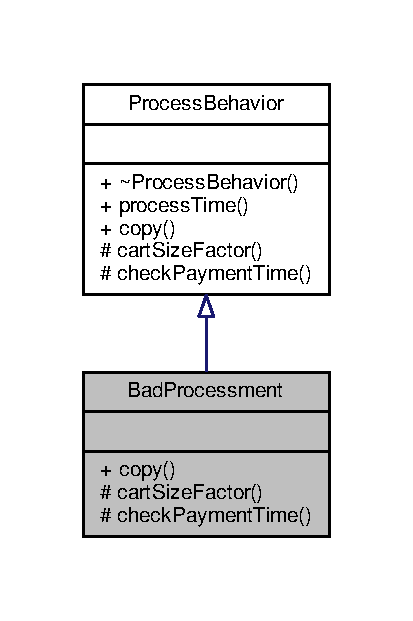
\includegraphics[width=198pt]{classBadProcessment__inherit__graph}
\end{center}
\end{figure}


Collaboration diagram for Bad\-Processment\-:\nopagebreak
\begin{figure}[H]
\begin{center}
\leavevmode
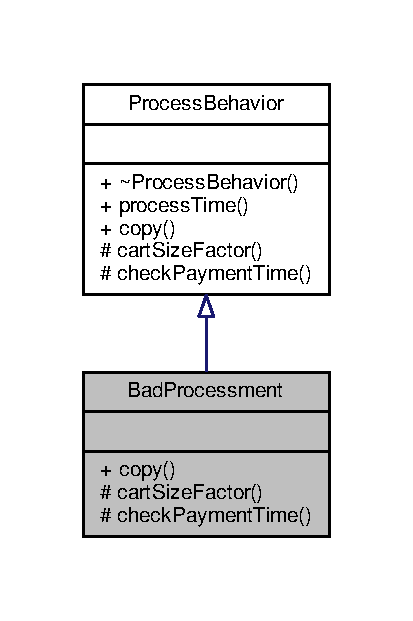
\includegraphics[width=198pt]{classBadProcessment__coll__graph}
\end{center}
\end{figure}
\subsection*{Public Member Functions}
\begin{DoxyCompactItemize}
\item 
\hyperlink{classProcessBehavior}{Process\-Behavior} $\ast$ \hyperlink{classBadProcessment_a682870ce18151f42f864fd22ab61363f}{copy} () const 
\begin{DoxyCompactList}\small\item\em Calcula o tempo de saída do cliente recebido. \end{DoxyCompactList}\end{DoxyCompactItemize}
\subsection*{Protected Member Functions}
\begin{DoxyCompactItemize}
\item 
int \hyperlink{classBadProcessment_a921c2f0f7fa59d0f92a35ddc440eeffb}{cart\-Size\-Factor} ()
\item 
int \hyperlink{classBadProcessment_aba28469024834d364c3d599436732204}{check\-Payment\-Time} ()
\end{DoxyCompactItemize}


\subsection{Member Function Documentation}
\hypertarget{classBadProcessment_a921c2f0f7fa59d0f92a35ddc440eeffb}{\index{Bad\-Processment@{Bad\-Processment}!cart\-Size\-Factor@{cart\-Size\-Factor}}
\index{cart\-Size\-Factor@{cart\-Size\-Factor}!BadProcessment@{Bad\-Processment}}
\subsubsection[{cart\-Size\-Factor}]{\setlength{\rightskip}{0pt plus 5cm}int Bad\-Processment\-::cart\-Size\-Factor (
\begin{DoxyParamCaption}
{}
\end{DoxyParamCaption}
)\hspace{0.3cm}{\ttfamily [protected]}, {\ttfamily [virtual]}}}\label{classBadProcessment_a921c2f0f7fa59d0f92a35ddc440eeffb}


Implements \hyperlink{classProcessBehavior_a7ccbf0f5499819a6f6c524bfd8595921}{Process\-Behavior}.

\hypertarget{classBadProcessment_aba28469024834d364c3d599436732204}{\index{Bad\-Processment@{Bad\-Processment}!check\-Payment\-Time@{check\-Payment\-Time}}
\index{check\-Payment\-Time@{check\-Payment\-Time}!BadProcessment@{Bad\-Processment}}
\subsubsection[{check\-Payment\-Time}]{\setlength{\rightskip}{0pt plus 5cm}int Bad\-Processment\-::check\-Payment\-Time (
\begin{DoxyParamCaption}
{}
\end{DoxyParamCaption}
)\hspace{0.3cm}{\ttfamily [protected]}, {\ttfamily [virtual]}}}\label{classBadProcessment_aba28469024834d364c3d599436732204}


Implements \hyperlink{classProcessBehavior_ac3e63322c133f11387759d34dd8fb13c}{Process\-Behavior}.

\hypertarget{classBadProcessment_a682870ce18151f42f864fd22ab61363f}{\index{Bad\-Processment@{Bad\-Processment}!copy@{copy}}
\index{copy@{copy}!BadProcessment@{Bad\-Processment}}
\subsubsection[{copy}]{\setlength{\rightskip}{0pt plus 5cm}{\bf Process\-Behavior} $\ast$ Bad\-Processment\-::copy (
\begin{DoxyParamCaption}
{}
\end{DoxyParamCaption}
) const\hspace{0.3cm}{\ttfamily [virtual]}}}\label{classBadProcessment_a682870ce18151f42f864fd22ab61363f}


Calcula o tempo de saída do cliente recebido. 

Esta é a implementação do caixa com processamento ruim


\begin{DoxyParams}{Parameters}
{\em Cliente} & que terá seu tempo de saída calculado\\
\hline
\end{DoxyParams}
\begin{DoxyReturn}{Returns}
O horário que esse cliente sairá do supermercado 
\end{DoxyReturn}


Implements \hyperlink{classProcessBehavior_afec2ad87efbdc778a93c7e692c97878e}{Process\-Behavior}.



The documentation for this class was generated from the following files\-:\begin{DoxyCompactItemize}
\item 
cashier/\hyperlink{BadProcessment_8h}{Bad\-Processment.\-h}\item 
cashier/\hyperlink{BadProcessment_8cpp}{Bad\-Processment.\-cpp}\end{DoxyCompactItemize}

\hypertarget{classCashier}{\section{Referência à classe Cashier}
\label{de/d14/classCashier}\index{Cashier@{Cashier}}
}
\subsection*{Membros públicos}
\begin{DoxyCompactItemize}
\item 
\hypertarget{classCashier_ae0b9b991bed233e91d802ed24a1689a0}{{\bfseries Cashier} (std\-::string id, double salary, const \hyperlink{classProcessBehavior}{Process\-Behavior} \&process\-Behavior, int time\-Of\-Arrival, bool over\-Time)}\label{de/d14/classCashier_ae0b9b991bed233e91d802ed24a1689a0}

\item 
\hypertarget{classCashier_aa3438cc7699379f97fb86204cee96f3b}{{\bfseries Cashier} (const \hyperlink{classCashier}{Cashier} \&other)}\label{de/d14/classCashier_aa3438cc7699379f97fb86204cee96f3b}

\item 
\hypertarget{classCashier_ae50bc394e4ac4ee80817aff2b8ecd846}{\hyperlink{classCashier}{Cashier} \& {\bfseries operator=} (\hyperlink{classCashier}{Cashier} other)}\label{de/d14/classCashier_ae50bc394e4ac4ee80817aff2b8ecd846}

\item 
\hypertarget{classCashier_a8a0e504ffb0178331eac83900182de06}{void {\bfseries add\-Client} (\hyperlink{classClient}{Client} \&client)}\label{de/d14/classCashier_a8a0e504ffb0178331eac83900182de06}

\item 
\hypertarget{classCashier_ae84eef690ba7beb9c38e1813bf4a4934}{void {\bfseries update} (int current\-Time)}\label{de/d14/classCashier_ae84eef690ba7beb9c38e1813bf4a4934}

\item 
\hypertarget{classCashier_a21fec12d0be5f4ae5f530ff0ee0d6c6e}{double {\bfseries total\-Income} () const }\label{de/d14/classCashier_a21fec12d0be5f4ae5f530ff0ee0d6c6e}

\item 
\hypertarget{classCashier_aef70a7f98c9049e74830abdc3ef16e48}{double {\bfseries average\-Income} () const }\label{de/d14/classCashier_aef70a7f98c9049e74830abdc3ef16e48}

\item 
\hypertarget{classCashier_af627f5b03558df68531aa86e4eced5a2}{int {\bfseries total\-Waiting\-Time} () const }\label{de/d14/classCashier_af627f5b03558df68531aa86e4eced5a2}

\item 
\hypertarget{classCashier_ae6d59b96dd0a97414a883056487f9934}{int {\bfseries clients\-Served} () const }\label{de/d14/classCashier_ae6d59b96dd0a97414a883056487f9934}

\item 
\hypertarget{classCashier_a6c4e3d00ebeb1e9af88feb6ff2285369}{int {\bfseries queue\-Size} () const }\label{de/d14/classCashier_a6c4e3d00ebeb1e9af88feb6ff2285369}

\item 
\hypertarget{classCashier_a20019398d52b20997fa109228268b583}{int {\bfseries num\-Of\-Items} () const }\label{de/d14/classCashier_a20019398d52b20997fa109228268b583}

\item 
\hypertarget{classCashier_a5c32d6426d9e272649151a965564afb1}{std\-::string {\bfseries id} () const }\label{de/d14/classCashier_a5c32d6426d9e272649151a965564afb1}

\item 
\hypertarget{classCashier_ad394576caf7eb468ce5684181b53c83f}{double {\bfseries salary} () const }\label{de/d14/classCashier_ad394576caf7eb468ce5684181b53c83f}

\item 
\hypertarget{classCashier_ac0bc4c8f7d5317f296a6ed103a75dfe4}{int {\bfseries time\-Of\-Arrival} () const }\label{de/d14/classCashier_ac0bc4c8f7d5317f296a6ed103a75dfe4}

\item 
\hypertarget{classCashier_a61d85cd680cc3611c5e9fa6d12544236}{bool {\bfseries over\-Time} () const }\label{de/d14/classCashier_a61d85cd680cc3611c5e9fa6d12544236}

\end{DoxyCompactItemize}
\subsection*{Amigos}
\begin{DoxyCompactItemize}
\item 
\hypertarget{classCashier_a34bcc8f6f2057300c0eba451506915d1}{void {\bfseries swap} (\hyperlink{classCashier}{Cashier} \&first, \hyperlink{classCashier}{Cashier} \&second)}\label{de/d14/classCashier_a34bcc8f6f2057300c0eba451506915d1}

\end{DoxyCompactItemize}


A documentação para esta classe foi gerada a partir dos seguintes ficheiros\-:\begin{DoxyCompactItemize}
\item 
cashier/Cashier.\-h\item 
cashier/Cashier.\-cpp\end{DoxyCompactItemize}

\hypertarget{classClient}{\section{Referência à classe Client}
\label{d1/d37/classClient}\index{Client@{Client}}
}
\subsection*{Membros públicos}
\begin{DoxyCompactItemize}
\item 
\hypertarget{classClient_a3b5a8f683ebd0abdf91b8cfe4c8be817}{{\bfseries Client} (const \hyperlink{classSearchBehavior}{Search\-Behavior} \&search\-Behavior, Payment\-Type payment\-Type, int time\-Of\-Arrival, int cart\-Size, double cart\-Value)}\label{d1/d37/classClient_a3b5a8f683ebd0abdf91b8cfe4c8be817}

\item 
\hypertarget{classClient_a4d8e3b9fdfa24b7586bcf24537b89b67}{{\bfseries Client} (const \hyperlink{classClient}{Client} \&other)}\label{d1/d37/classClient_a4d8e3b9fdfa24b7586bcf24537b89b67}

\item 
\hypertarget{classClient_acc35776f6a75d2fb8d4abfb3cc33f8a3}{\hyperlink{classClient}{Client} \& {\bfseries operator=} (\hyperlink{classClient}{Client} other)}\label{d1/d37/classClient_acc35776f6a75d2fb8d4abfb3cc33f8a3}

\item 
\hypertarget{classClient_a2ef5728c74cc7f9dfce8b5e9e950427c}{int {\bfseries cart\-Size} () const }\label{d1/d37/classClient_a2ef5728c74cc7f9dfce8b5e9e950427c}

\item 
\hypertarget{classClient_a52b9e8ce7f11c440fb532f6056db5fe2}{double {\bfseries cart\-Value} () const }\label{d1/d37/classClient_a52b9e8ce7f11c440fb532f6056db5fe2}

\item 
\hypertarget{classClient_a9cceb950fc9c53ea35bcddf6214e4e4f}{Payment\-Type {\bfseries payment\-Type} () const }\label{d1/d37/classClient_a9cceb950fc9c53ea35bcddf6214e4e4f}

\item 
\hypertarget{classClient_ae56c063a8bc1c57e9c47ad88b1770994}{int {\bfseries time\-Of\-Departure} () const }\label{d1/d37/classClient_ae56c063a8bc1c57e9c47ad88b1770994}

\item 
\hypertarget{classClient_af327f525b4cf7838d97c095c8dd00e60}{int {\bfseries time\-Of\-Arrival} () const }\label{d1/d37/classClient_af327f525b4cf7838d97c095c8dd00e60}

\item 
\hypertarget{classClient_a282e19d2e25da6d8ee8a5c8ad5f0bdd7}{void {\bfseries time\-Of\-Departure} (int time\-Of\-Departure)}\label{d1/d37/classClient_a282e19d2e25da6d8ee8a5c8ad5f0bdd7}

\item 
\hypertarget{classClient_a7d60abe00b79e6f09e113d00b47d2a03}{void {\bfseries choose\-Cashier} (std\-::vector$<$ \hyperlink{classCashier}{Cashier} $>$ \&cashiers)}\label{d1/d37/classClient_a7d60abe00b79e6f09e113d00b47d2a03}

\end{DoxyCompactItemize}
\subsection*{Amigos}
\begin{DoxyCompactItemize}
\item 
\hypertarget{classClient_a359e644998b9e1c2adf9d9afe3e04d8c}{void {\bfseries swap} (\hyperlink{classClient}{Client} \&first, \hyperlink{classClient}{Client} \&second)}\label{d1/d37/classClient_a359e644998b9e1c2adf9d9afe3e04d8c}

\end{DoxyCompactItemize}


A documentação para esta classe foi gerada a partir dos seguintes ficheiros\-:\begin{DoxyCompactItemize}
\item 
client/Client.\-h\item 
client/Client.\-cpp\end{DoxyCompactItemize}

\hypertarget{classGoodProcessment}{\section{Good\-Processment Class Reference}
\label{classGoodProcessment}\index{Good\-Processment@{Good\-Processment}}
}


{\ttfamily \#include $<$Good\-Processment.\-h$>$}



Inheritance diagram for Good\-Processment\-:\nopagebreak
\begin{figure}[H]
\begin{center}
\leavevmode
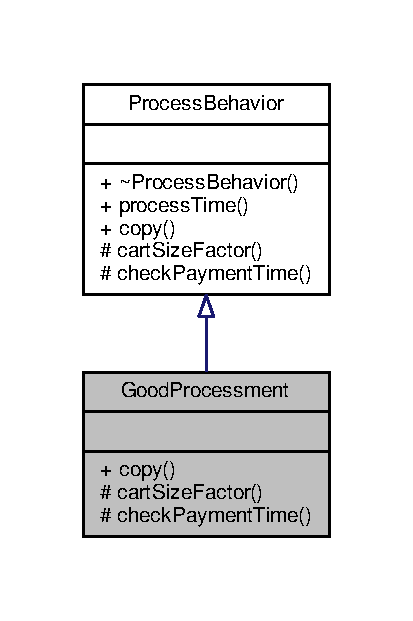
\includegraphics[width=198pt]{classGoodProcessment__inherit__graph}
\end{center}
\end{figure}


Collaboration diagram for Good\-Processment\-:\nopagebreak
\begin{figure}[H]
\begin{center}
\leavevmode
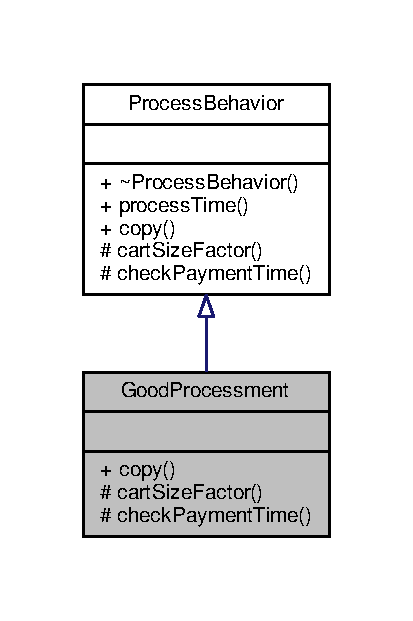
\includegraphics[width=198pt]{classGoodProcessment__coll__graph}
\end{center}
\end{figure}
\subsection*{Public Member Functions}
\begin{DoxyCompactItemize}
\item 
\hyperlink{classProcessBehavior}{Process\-Behavior} $\ast$ \hyperlink{classGoodProcessment_a1c2dfca6ae6c4ab034dfcfc423bf338b}{copy} () const 
\begin{DoxyCompactList}\small\item\em Calcula o tempo de saída do cliente recebido. \end{DoxyCompactList}\end{DoxyCompactItemize}
\subsection*{Protected Member Functions}
\begin{DoxyCompactItemize}
\item 
int \hyperlink{classGoodProcessment_a99170ba3993e1511cc1fa82aba883bbc}{cart\-Size\-Factor} ()
\item 
int \hyperlink{classGoodProcessment_a126bda449e47094c49f501dcb0cb5d88}{check\-Payment\-Time} ()
\end{DoxyCompactItemize}


\subsection{Member Function Documentation}
\hypertarget{classGoodProcessment_a99170ba3993e1511cc1fa82aba883bbc}{\index{Good\-Processment@{Good\-Processment}!cart\-Size\-Factor@{cart\-Size\-Factor}}
\index{cart\-Size\-Factor@{cart\-Size\-Factor}!GoodProcessment@{Good\-Processment}}
\subsubsection[{cart\-Size\-Factor}]{\setlength{\rightskip}{0pt plus 5cm}int Good\-Processment\-::cart\-Size\-Factor (
\begin{DoxyParamCaption}
{}
\end{DoxyParamCaption}
)\hspace{0.3cm}{\ttfamily [protected]}, {\ttfamily [virtual]}}}\label{classGoodProcessment_a99170ba3993e1511cc1fa82aba883bbc}


Implements \hyperlink{classProcessBehavior_a7ccbf0f5499819a6f6c524bfd8595921}{Process\-Behavior}.

\hypertarget{classGoodProcessment_a126bda449e47094c49f501dcb0cb5d88}{\index{Good\-Processment@{Good\-Processment}!check\-Payment\-Time@{check\-Payment\-Time}}
\index{check\-Payment\-Time@{check\-Payment\-Time}!GoodProcessment@{Good\-Processment}}
\subsubsection[{check\-Payment\-Time}]{\setlength{\rightskip}{0pt plus 5cm}int Good\-Processment\-::check\-Payment\-Time (
\begin{DoxyParamCaption}
{}
\end{DoxyParamCaption}
)\hspace{0.3cm}{\ttfamily [protected]}, {\ttfamily [virtual]}}}\label{classGoodProcessment_a126bda449e47094c49f501dcb0cb5d88}


Implements \hyperlink{classProcessBehavior_ac3e63322c133f11387759d34dd8fb13c}{Process\-Behavior}.

\hypertarget{classGoodProcessment_a1c2dfca6ae6c4ab034dfcfc423bf338b}{\index{Good\-Processment@{Good\-Processment}!copy@{copy}}
\index{copy@{copy}!GoodProcessment@{Good\-Processment}}
\subsubsection[{copy}]{\setlength{\rightskip}{0pt plus 5cm}{\bf Process\-Behavior} $\ast$ Good\-Processment\-::copy (
\begin{DoxyParamCaption}
{}
\end{DoxyParamCaption}
) const\hspace{0.3cm}{\ttfamily [virtual]}}}\label{classGoodProcessment_a1c2dfca6ae6c4ab034dfcfc423bf338b}


Calcula o tempo de saída do cliente recebido. 

Esta é a implementação do caixa com processamento bom


\begin{DoxyParams}{Parameters}
{\em Cliente} & que terá seu tempo de saída calculado\\
\hline
\end{DoxyParams}
\begin{DoxyReturn}{Returns}
O horário que esse cliente sairá do supermercado 
\end{DoxyReturn}


Implements \hyperlink{classProcessBehavior_afec2ad87efbdc778a93c7e692c97878e}{Process\-Behavior}.



The documentation for this class was generated from the following files\-:\begin{DoxyCompactItemize}
\item 
cashier/\hyperlink{GoodProcessment_8h}{Good\-Processment.\-h}\item 
cashier/\hyperlink{GoodProcessment_8cpp}{Good\-Processment.\-cpp}\end{DoxyCompactItemize}

\hypertarget{classMediumProcessment}{\section{Medium\-Processment Class Reference}
\label{classMediumProcessment}\index{Medium\-Processment@{Medium\-Processment}}
}


{\ttfamily \#include $<$Medium\-Processment.\-h$>$}



Inheritance diagram for Medium\-Processment\-:\nopagebreak
\begin{figure}[H]
\begin{center}
\leavevmode
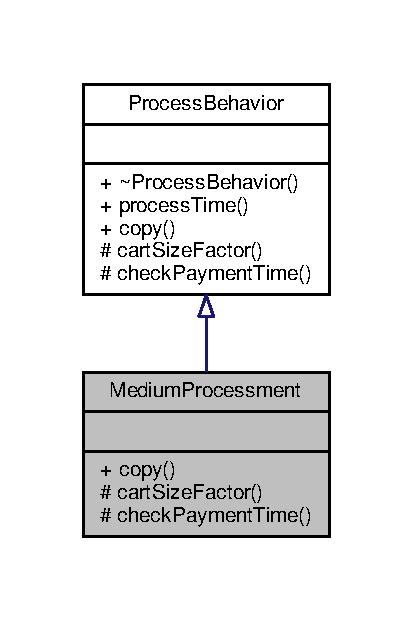
\includegraphics[width=198pt]{classMediumProcessment__inherit__graph}
\end{center}
\end{figure}


Collaboration diagram for Medium\-Processment\-:\nopagebreak
\begin{figure}[H]
\begin{center}
\leavevmode
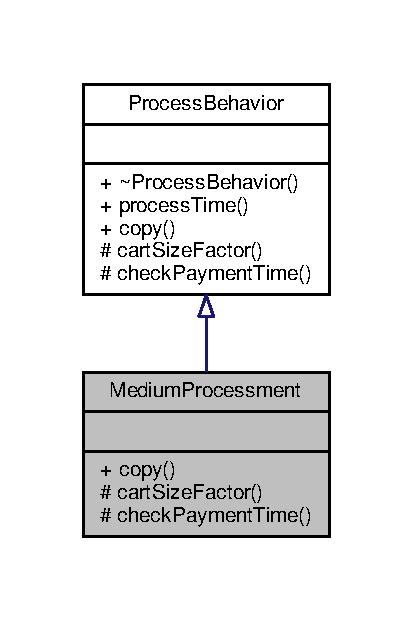
\includegraphics[width=198pt]{classMediumProcessment__coll__graph}
\end{center}
\end{figure}
\subsection*{Public Member Functions}
\begin{DoxyCompactItemize}
\item 
\hyperlink{classProcessBehavior}{Process\-Behavior} $\ast$ \hyperlink{classMediumProcessment_a8207750eb9bf65f830770b3631845934}{copy} () const 
\begin{DoxyCompactList}\small\item\em Calcula o tempo de saída do cliente recebido. \end{DoxyCompactList}\end{DoxyCompactItemize}
\subsection*{Protected Member Functions}
\begin{DoxyCompactItemize}
\item 
int \hyperlink{classMediumProcessment_a8baac43e0224353f4c5340c5e7117b62}{cart\-Size\-Factor} ()
\item 
int \hyperlink{classMediumProcessment_ab14abd8ec6b6a7af6aa2879c471dded7}{check\-Payment\-Time} ()
\end{DoxyCompactItemize}


\subsection{Member Function Documentation}
\hypertarget{classMediumProcessment_a8baac43e0224353f4c5340c5e7117b62}{\index{Medium\-Processment@{Medium\-Processment}!cart\-Size\-Factor@{cart\-Size\-Factor}}
\index{cart\-Size\-Factor@{cart\-Size\-Factor}!MediumProcessment@{Medium\-Processment}}
\subsubsection[{cart\-Size\-Factor}]{\setlength{\rightskip}{0pt plus 5cm}int Medium\-Processment\-::cart\-Size\-Factor (
\begin{DoxyParamCaption}
{}
\end{DoxyParamCaption}
)\hspace{0.3cm}{\ttfamily [protected]}, {\ttfamily [virtual]}}}\label{classMediumProcessment_a8baac43e0224353f4c5340c5e7117b62}


Implements \hyperlink{classProcessBehavior_a7ccbf0f5499819a6f6c524bfd8595921}{Process\-Behavior}.

\hypertarget{classMediumProcessment_ab14abd8ec6b6a7af6aa2879c471dded7}{\index{Medium\-Processment@{Medium\-Processment}!check\-Payment\-Time@{check\-Payment\-Time}}
\index{check\-Payment\-Time@{check\-Payment\-Time}!MediumProcessment@{Medium\-Processment}}
\subsubsection[{check\-Payment\-Time}]{\setlength{\rightskip}{0pt plus 5cm}int Medium\-Processment\-::check\-Payment\-Time (
\begin{DoxyParamCaption}
{}
\end{DoxyParamCaption}
)\hspace{0.3cm}{\ttfamily [protected]}, {\ttfamily [virtual]}}}\label{classMediumProcessment_ab14abd8ec6b6a7af6aa2879c471dded7}


Implements \hyperlink{classProcessBehavior_ac3e63322c133f11387759d34dd8fb13c}{Process\-Behavior}.

\hypertarget{classMediumProcessment_a8207750eb9bf65f830770b3631845934}{\index{Medium\-Processment@{Medium\-Processment}!copy@{copy}}
\index{copy@{copy}!MediumProcessment@{Medium\-Processment}}
\subsubsection[{copy}]{\setlength{\rightskip}{0pt plus 5cm}{\bf Process\-Behavior} $\ast$ Medium\-Processment\-::copy (
\begin{DoxyParamCaption}
{}
\end{DoxyParamCaption}
) const\hspace{0.3cm}{\ttfamily [virtual]}}}\label{classMediumProcessment_a8207750eb9bf65f830770b3631845934}


Calcula o tempo de saída do cliente recebido. 

Esta é a implementação do caixa com processamento médio


\begin{DoxyParams}{Parameters}
{\em Cliente} & que terá seu tempo de saída calculado\\
\hline
\end{DoxyParams}
\begin{DoxyReturn}{Returns}
O horário que esse cliente sairá do supermercado 
\end{DoxyReturn}


Implements \hyperlink{classProcessBehavior_afec2ad87efbdc778a93c7e692c97878e}{Process\-Behavior}.



The documentation for this class was generated from the following files\-:\begin{DoxyCompactItemize}
\item 
cashier/\hyperlink{MediumProcessment_8h}{Medium\-Processment.\-h}\item 
cashier/\hyperlink{MediumProcessment_8cpp}{Medium\-Processment.\-cpp}\end{DoxyCompactItemize}

\hypertarget{classProcessBehavior}{\section{Process\-Behavior Class Reference}
\label{classProcessBehavior}\index{Process\-Behavior@{Process\-Behavior}}
}


{\ttfamily \#include $<$Process\-Behavior.\-h$>$}



Inheritance diagram for Process\-Behavior\-:\nopagebreak
\begin{figure}[H]
\begin{center}
\leavevmode
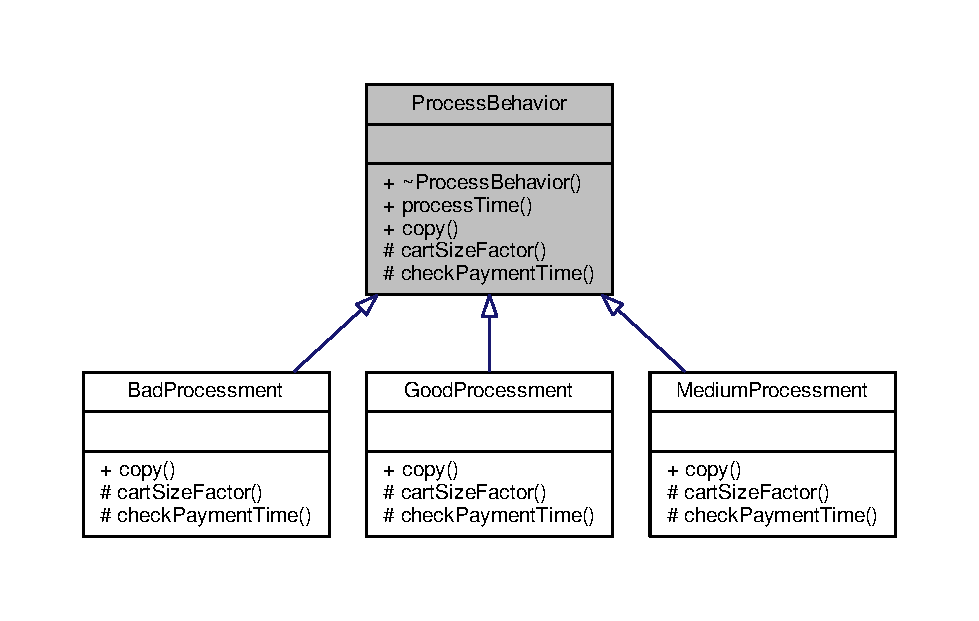
\includegraphics[width=350pt]{classProcessBehavior__inherit__graph}
\end{center}
\end{figure}


Collaboration diagram for Process\-Behavior\-:\nopagebreak
\begin{figure}[H]
\begin{center}
\leavevmode
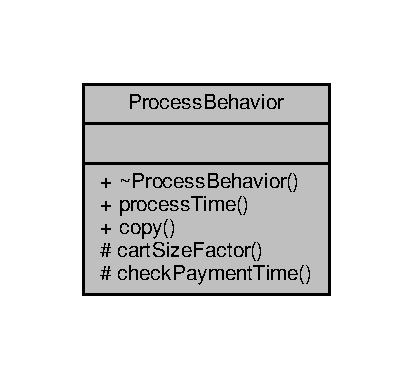
\includegraphics[width=198pt]{classProcessBehavior__coll__graph}
\end{center}
\end{figure}
\subsection*{Public Member Functions}
\begin{DoxyCompactItemize}
\item 
virtual \hyperlink{classProcessBehavior_acd6a6ace48909139c252358d67dc94ea}{$\sim$\-Process\-Behavior} ()
\item 
int \hyperlink{classProcessBehavior_a17faac1683e9da239d33026db1fd11f8}{process\-Time} (const \hyperlink{classClient}{Client} \&client)
\begin{DoxyCompactList}\small\item\em Calcula o tempo de saída do cliente recebido. \end{DoxyCompactList}\item 
virtual \hyperlink{classProcessBehavior}{Process\-Behavior} $\ast$ \hyperlink{classProcessBehavior_afec2ad87efbdc778a93c7e692c97878e}{copy} () const =0
\end{DoxyCompactItemize}
\subsection*{Protected Member Functions}
\begin{DoxyCompactItemize}
\item 
virtual int \hyperlink{classProcessBehavior_a7ccbf0f5499819a6f6c524bfd8595921}{cart\-Size\-Factor} ()=0
\item 
virtual int \hyperlink{classProcessBehavior_ac3e63322c133f11387759d34dd8fb13c}{check\-Payment\-Time} ()=0
\end{DoxyCompactItemize}


\subsection{Constructor \& Destructor Documentation}
\hypertarget{classProcessBehavior_acd6a6ace48909139c252358d67dc94ea}{\index{Process\-Behavior@{Process\-Behavior}!$\sim$\-Process\-Behavior@{$\sim$\-Process\-Behavior}}
\index{$\sim$\-Process\-Behavior@{$\sim$\-Process\-Behavior}!ProcessBehavior@{Process\-Behavior}}
\subsubsection[{$\sim$\-Process\-Behavior}]{\setlength{\rightskip}{0pt plus 5cm}virtual Process\-Behavior\-::$\sim$\-Process\-Behavior (
\begin{DoxyParamCaption}
{}
\end{DoxyParamCaption}
)\hspace{0.3cm}{\ttfamily [inline]}, {\ttfamily [virtual]}}}\label{classProcessBehavior_acd6a6ace48909139c252358d67dc94ea}


\subsection{Member Function Documentation}
\hypertarget{classProcessBehavior_a7ccbf0f5499819a6f6c524bfd8595921}{\index{Process\-Behavior@{Process\-Behavior}!cart\-Size\-Factor@{cart\-Size\-Factor}}
\index{cart\-Size\-Factor@{cart\-Size\-Factor}!ProcessBehavior@{Process\-Behavior}}
\subsubsection[{cart\-Size\-Factor}]{\setlength{\rightskip}{0pt plus 5cm}virtual int Process\-Behavior\-::cart\-Size\-Factor (
\begin{DoxyParamCaption}
{}
\end{DoxyParamCaption}
)\hspace{0.3cm}{\ttfamily [protected]}, {\ttfamily [pure virtual]}}}\label{classProcessBehavior_a7ccbf0f5499819a6f6c524bfd8595921}


Implemented in \hyperlink{classBadProcessment_a921c2f0f7fa59d0f92a35ddc440eeffb}{Bad\-Processment}, \hyperlink{classGoodProcessment_a99170ba3993e1511cc1fa82aba883bbc}{Good\-Processment}, and \hyperlink{classMediumProcessment_a8baac43e0224353f4c5340c5e7117b62}{Medium\-Processment}.

\hypertarget{classProcessBehavior_ac3e63322c133f11387759d34dd8fb13c}{\index{Process\-Behavior@{Process\-Behavior}!check\-Payment\-Time@{check\-Payment\-Time}}
\index{check\-Payment\-Time@{check\-Payment\-Time}!ProcessBehavior@{Process\-Behavior}}
\subsubsection[{check\-Payment\-Time}]{\setlength{\rightskip}{0pt plus 5cm}virtual int Process\-Behavior\-::check\-Payment\-Time (
\begin{DoxyParamCaption}
{}
\end{DoxyParamCaption}
)\hspace{0.3cm}{\ttfamily [protected]}, {\ttfamily [pure virtual]}}}\label{classProcessBehavior_ac3e63322c133f11387759d34dd8fb13c}


Implemented in \hyperlink{classBadProcessment_aba28469024834d364c3d599436732204}{Bad\-Processment}, \hyperlink{classGoodProcessment_a126bda449e47094c49f501dcb0cb5d88}{Good\-Processment}, and \hyperlink{classMediumProcessment_ab14abd8ec6b6a7af6aa2879c471dded7}{Medium\-Processment}.

\hypertarget{classProcessBehavior_afec2ad87efbdc778a93c7e692c97878e}{\index{Process\-Behavior@{Process\-Behavior}!copy@{copy}}
\index{copy@{copy}!ProcessBehavior@{Process\-Behavior}}
\subsubsection[{copy}]{\setlength{\rightskip}{0pt plus 5cm}virtual {\bf Process\-Behavior}$\ast$ Process\-Behavior\-::copy (
\begin{DoxyParamCaption}
{}
\end{DoxyParamCaption}
) const\hspace{0.3cm}{\ttfamily [pure virtual]}}}\label{classProcessBehavior_afec2ad87efbdc778a93c7e692c97878e}


Implemented in \hyperlink{classBadProcessment_a682870ce18151f42f864fd22ab61363f}{Bad\-Processment}, \hyperlink{classGoodProcessment_a1c2dfca6ae6c4ab034dfcfc423bf338b}{Good\-Processment}, and \hyperlink{classMediumProcessment_a8207750eb9bf65f830770b3631845934}{Medium\-Processment}.

\hypertarget{classProcessBehavior_a17faac1683e9da239d33026db1fd11f8}{\index{Process\-Behavior@{Process\-Behavior}!process\-Time@{process\-Time}}
\index{process\-Time@{process\-Time}!ProcessBehavior@{Process\-Behavior}}
\subsubsection[{process\-Time}]{\setlength{\rightskip}{0pt plus 5cm}int Process\-Behavior\-::process\-Time (
\begin{DoxyParamCaption}
\item[{const {\bf Client} \&}]{client}
\end{DoxyParamCaption}
)}}\label{classProcessBehavior_a17faac1683e9da239d33026db1fd11f8}


Calcula o tempo de saída do cliente recebido. 

Utilizando a implementação do caixa do comportamento de processamento de clientes, calcula o tempo de saída do cliente Existem 3 implementações diferentes. Processamento bom, médio e ruim. O que interfere no tempo de processamento.


\begin{DoxyParams}{Parameters}
{\em Cliente} & que terá seu tempo de saída calculado\\
\hline
\end{DoxyParams}
\begin{DoxyReturn}{Returns}
O horário que esse cliente sairá do supermercado 
\end{DoxyReturn}


The documentation for this class was generated from the following files\-:\begin{DoxyCompactItemize}
\item 
cashier/\hyperlink{ProcessBehavior_8h}{Process\-Behavior.\-h}\item 
cashier/\hyperlink{ProcessBehavior_8cpp}{Process\-Behavior.\-cpp}\end{DoxyCompactItemize}

\hypertarget{classQueue}{\section{Queue$<$ T $>$ Class Template Reference}
\label{classQueue}\index{Queue$<$ T $>$@{Queue$<$ T $>$}}
}
\subsection*{Public Types}
\begin{DoxyCompactItemize}
\item 
\hypertarget{classQueue_abc9e9289124dc3ae5377a7e3d3fbe928}{typedef iterator\-\_\-base$<$ T $>$ {\bfseries iterator}}\label{classQueue_abc9e9289124dc3ae5377a7e3d3fbe928}

\item 
\hypertarget{classQueue_a10a22f024abb831966e98b859bb2e64d}{typedef iterator\-\_\-base$<$ const T $>$ {\bfseries const\-\_\-iterator}}\label{classQueue_a10a22f024abb831966e98b859bb2e64d}

\item 
\hypertarget{classQueue_abc9e9289124dc3ae5377a7e3d3fbe928}{typedef iterator\-\_\-base$<$ T $>$ {\bfseries iterator}}\label{classQueue_abc9e9289124dc3ae5377a7e3d3fbe928}

\item 
\hypertarget{classQueue_a10a22f024abb831966e98b859bb2e64d}{typedef iterator\-\_\-base$<$ const T $>$ {\bfseries const\-\_\-iterator}}\label{classQueue_a10a22f024abb831966e98b859bb2e64d}

\end{DoxyCompactItemize}
\subsection*{Public Member Functions}
\begin{DoxyCompactItemize}
\item 
\hypertarget{classQueue_a3e03781c5f55e9f9ff862360aa33d9a9}{void {\bfseries push\-\_\-back} (const T \&info)}\label{classQueue_a3e03781c5f55e9f9ff862360aa33d9a9}

\item 
\hypertarget{classQueue_a01fbe357228d8f3d10c51def77f04647}{void {\bfseries push\-\_\-front} (const T \&dado)}\label{classQueue_a01fbe357228d8f3d10c51def77f04647}

\item 
\hypertarget{classQueue_a98c1f8cdb878cc1ad5d7f5dc13eec9b8}{void {\bfseries push} (int position, const T \&dado)}\label{classQueue_a98c1f8cdb878cc1ad5d7f5dc13eec9b8}

\item 
\hypertarget{classQueue_abeee018138cbb5226e5352a5788e23bd}{T {\bfseries pop} ()}\label{classQueue_abeee018138cbb5226e5352a5788e23bd}

\item 
\hypertarget{classQueue_a4836777845e48b56e4ddf04b3da677c9}{T {\bfseries pop} (int posicao)}\label{classQueue_a4836777845e48b56e4ddf04b3da677c9}

\item 
\hypertarget{classQueue_a91492afa6103be0ffdfcc886fc996b25}{T {\bfseries at} (int position) const }\label{classQueue_a91492afa6103be0ffdfcc886fc996b25}

\item 
\hypertarget{classQueue_a74e1442a08f38177e7dd7f7c8af22d30}{bool {\bfseries empty} () const }\label{classQueue_a74e1442a08f38177e7dd7f7c8af22d30}

\item 
\hypertarget{classQueue_ad13b6467a10f5b6b8b78716787a77fd4}{int {\bfseries size} () const }\label{classQueue_ad13b6467a10f5b6b8b78716787a77fd4}

\item 
\hypertarget{classQueue_a0f8479ac20e00d122558dce6c3c71473}{iterator {\bfseries begin} ()}\label{classQueue_a0f8479ac20e00d122558dce6c3c71473}

\item 
\hypertarget{classQueue_aae0dd33cf275e880bc244aeba0f2fc25}{iterator {\bfseries end} ()}\label{classQueue_aae0dd33cf275e880bc244aeba0f2fc25}

\item 
\hypertarget{classQueue_a652c1526d0a99cc153bec8df86105cca}{const\-\_\-iterator {\bfseries begin} () const }\label{classQueue_a652c1526d0a99cc153bec8df86105cca}

\item 
\hypertarget{classQueue_abdd805a2bb752ed37ab2dbc1493a9e24}{const\-\_\-iterator {\bfseries end} () const }\label{classQueue_abdd805a2bb752ed37ab2dbc1493a9e24}

\item 
\hypertarget{classQueue_ac3b3b360bf22dd4ef5874449880ece63}{{\bfseries Queue} (const \hyperlink{classQueue}{Queue}$<$ T $>$ \&other)}\label{classQueue_ac3b3b360bf22dd4ef5874449880ece63}

\item 
\hypertarget{classQueue_ad683a72dcd5d34a7aa0b906aed09d32f}{void {\bfseries push\-\_\-back} (const T \&dado)}\label{classQueue_ad683a72dcd5d34a7aa0b906aed09d32f}

\item 
\hypertarget{classQueue_a21992fd19ab9b53682b03059ecd04c61}{T {\bfseries pop\-\_\-front} ()}\label{classQueue_a21992fd19ab9b53682b03059ecd04c61}

\item 
\hypertarget{classQueue_a91492afa6103be0ffdfcc886fc996b25}{T {\bfseries at} (int position) const }\label{classQueue_a91492afa6103be0ffdfcc886fc996b25}

\item 
\hypertarget{classQueue_ae9af6d3cfe017a2f1bf1fd35ce9e99c3}{T {\bfseries back} () const }\label{classQueue_ae9af6d3cfe017a2f1bf1fd35ce9e99c3}

\item 
\hypertarget{classQueue_a057aac4f78168ea144118dac4222d192}{T {\bfseries front} () const }\label{classQueue_a057aac4f78168ea144118dac4222d192}

\item 
\hypertarget{classQueue_a74e1442a08f38177e7dd7f7c8af22d30}{bool {\bfseries empty} () const }\label{classQueue_a74e1442a08f38177e7dd7f7c8af22d30}

\item 
\hypertarget{classQueue_ad13b6467a10f5b6b8b78716787a77fd4}{int {\bfseries size} () const }\label{classQueue_ad13b6467a10f5b6b8b78716787a77fd4}

\item 
\hypertarget{classQueue_a0f8479ac20e00d122558dce6c3c71473}{iterator {\bfseries begin} ()}\label{classQueue_a0f8479ac20e00d122558dce6c3c71473}

\item 
\hypertarget{classQueue_aae0dd33cf275e880bc244aeba0f2fc25}{iterator {\bfseries end} ()}\label{classQueue_aae0dd33cf275e880bc244aeba0f2fc25}

\item 
\hypertarget{classQueue_a652c1526d0a99cc153bec8df86105cca}{const\-\_\-iterator {\bfseries begin} () const }\label{classQueue_a652c1526d0a99cc153bec8df86105cca}

\item 
\hypertarget{classQueue_abdd805a2bb752ed37ab2dbc1493a9e24}{const\-\_\-iterator {\bfseries end} () const }\label{classQueue_abdd805a2bb752ed37ab2dbc1493a9e24}

\end{DoxyCompactItemize}


The documentation for this class was generated from the following files\-:\begin{DoxyCompactItemize}
\item 
data\-Structures/Circular\-List.\-h\item 
data\-Structures/Queue.\-h\end{DoxyCompactItemize}

\hypertarget{classSearchBehavior}{\section{Referência à classe Search\-Behavior}
\label{de/d9c/classSearchBehavior}\index{Search\-Behavior@{Search\-Behavior}}
}
Diagrama de heranças da classe Search\-Behavior\begin{figure}[H]
\begin{center}
\leavevmode
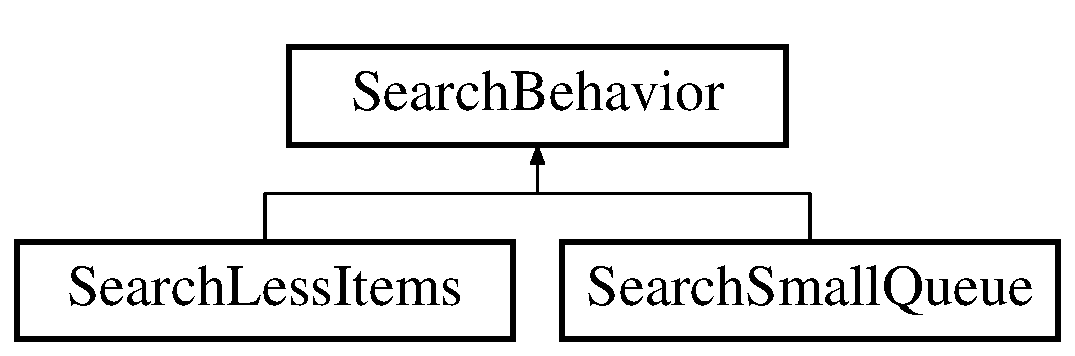
\includegraphics[height=2.000000cm]{de/d9c/classSearchBehavior}
\end{center}
\end{figure}
\subsection*{Membros públicos}
\begin{DoxyCompactItemize}
\item 
\hypertarget{classSearchBehavior_a66f39c53cb1cb9dc029c6fdae55c6234}{virtual \hyperlink{classSearchBehavior}{Search\-Behavior} $\ast$ {\bfseries copy} () const =0}\label{de/d9c/classSearchBehavior_a66f39c53cb1cb9dc029c6fdae55c6234}

\item 
\hypertarget{classSearchBehavior_a2347f04c014b7ad8ff9969b2cff6b126}{virtual \hyperlink{classCashier}{Cashier} \& {\bfseries search} (std\-::vector$<$ \hyperlink{classCashier}{Cashier} $>$ \&cashiers) const =0}\label{de/d9c/classSearchBehavior_a2347f04c014b7ad8ff9969b2cff6b126}

\end{DoxyCompactItemize}


A documentação para esta classe foi gerada a partir do seguinte ficheiro\-:\begin{DoxyCompactItemize}
\item 
client/Search\-Behavior.\-h\end{DoxyCompactItemize}

\hypertarget{classSearchLessItems}{\section{Referência à classe Search\-Less\-Items}
\label{df/d53/classSearchLessItems}\index{Search\-Less\-Items@{Search\-Less\-Items}}
}
Diagrama de heranças da classe Search\-Less\-Items\begin{figure}[H]
\begin{center}
\leavevmode
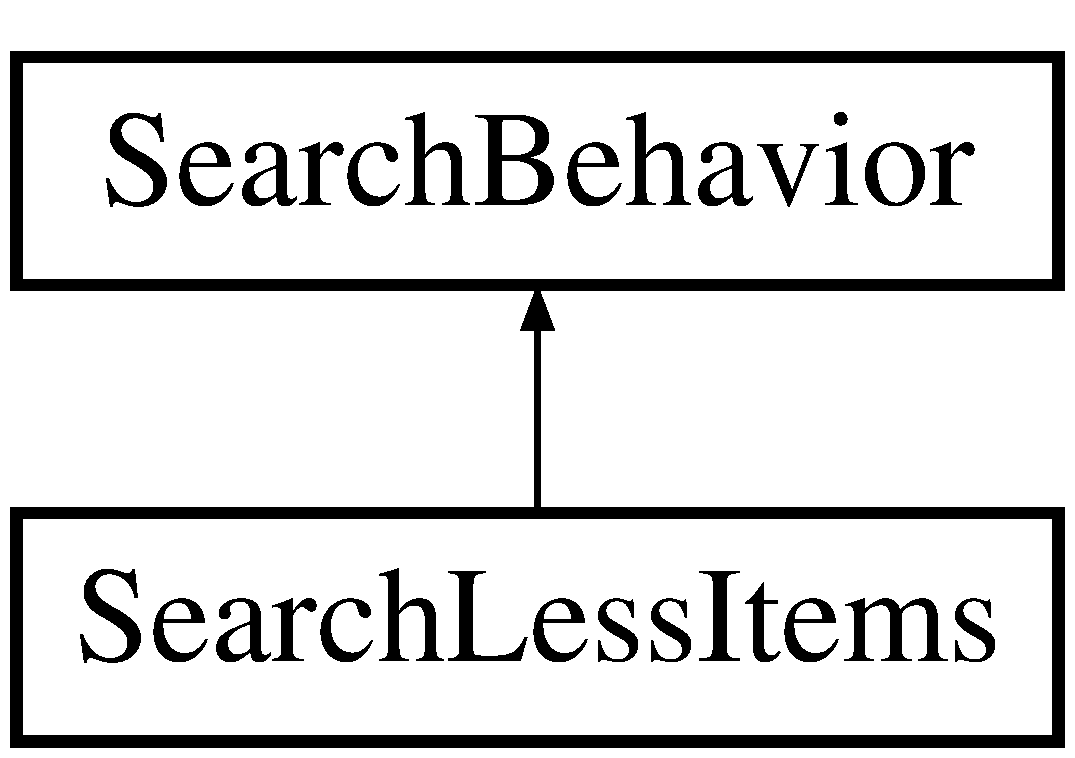
\includegraphics[height=2.000000cm]{df/d53/classSearchLessItems}
\end{center}
\end{figure}
\subsection*{Membros públicos}
\begin{DoxyCompactItemize}
\item 
\hypertarget{classSearchLessItems_a0f6334a5f52e56e6ee2ae2b40f4bf93a}{\hyperlink{classSearchBehavior}{Search\-Behavior} $\ast$ {\bfseries copy} () const }\label{df/d53/classSearchLessItems_a0f6334a5f52e56e6ee2ae2b40f4bf93a}

\item 
\hypertarget{classSearchLessItems_adc465fca95f9abee198f0aca23501369}{\hyperlink{classCashier}{Cashier} \& {\bfseries search} (std\-::vector$<$ \hyperlink{classCashier}{Cashier} $>$ \&cashiers) const }\label{df/d53/classSearchLessItems_adc465fca95f9abee198f0aca23501369}

\end{DoxyCompactItemize}


A documentação para esta classe foi gerada a partir dos seguintes ficheiros\-:\begin{DoxyCompactItemize}
\item 
client/Search\-Less\-Items.\-h\item 
client/Search\-Less\-Items.\-cpp\end{DoxyCompactItemize}

\hypertarget{classSearchSmallQueue}{\section{Referência à classe Search\-Small\-Queue}
\label{d3/d22/classSearchSmallQueue}\index{Search\-Small\-Queue@{Search\-Small\-Queue}}
}
Diagrama de heranças da classe Search\-Small\-Queue\begin{figure}[H]
\begin{center}
\leavevmode
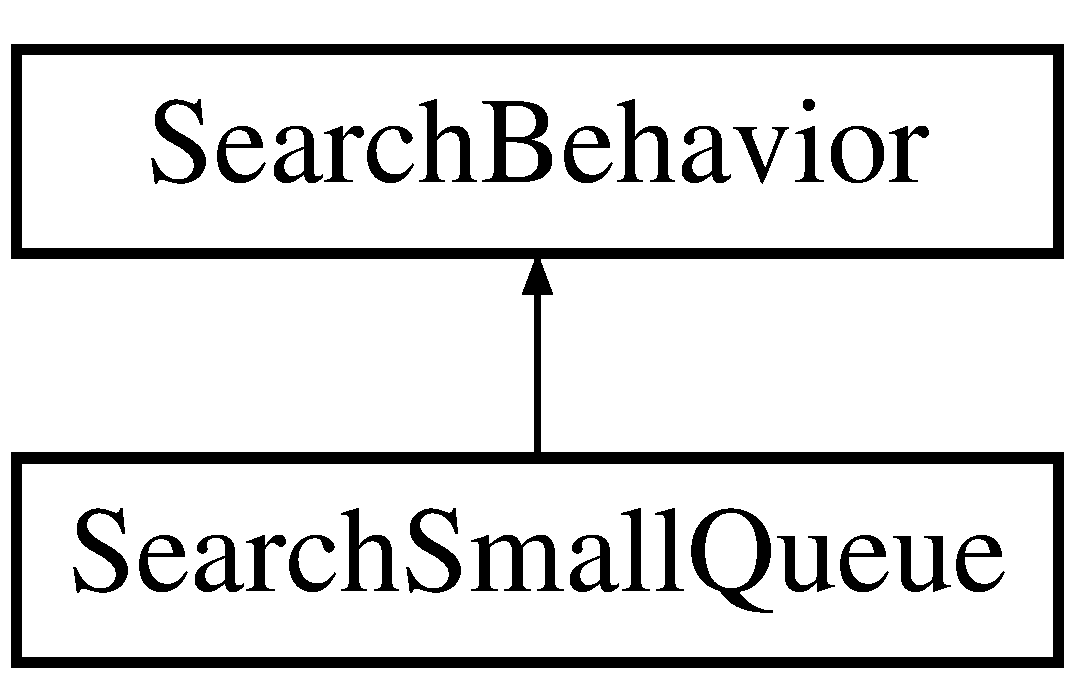
\includegraphics[height=2.000000cm]{d3/d22/classSearchSmallQueue}
\end{center}
\end{figure}
\subsection*{Membros públicos}
\begin{DoxyCompactItemize}
\item 
\hypertarget{classSearchSmallQueue_a060043acfc959d9fc046b99f19518401}{\hyperlink{classSearchBehavior}{Search\-Behavior} $\ast$ {\bfseries copy} () const }\label{d3/d22/classSearchSmallQueue_a060043acfc959d9fc046b99f19518401}

\item 
\hypertarget{classSearchSmallQueue_a78dabc28e376fdf7b38b75c31f46f9d1}{\hyperlink{classCashier}{Cashier} \& {\bfseries search} (std\-::vector$<$ \hyperlink{classCashier}{Cashier} $>$ \&cashiers) const }\label{d3/d22/classSearchSmallQueue_a78dabc28e376fdf7b38b75c31f46f9d1}

\end{DoxyCompactItemize}


A documentação para esta classe foi gerada a partir dos seguintes ficheiros\-:\begin{DoxyCompactItemize}
\item 
client/Search\-Small\-Queue.\-h\item 
client/Search\-Small\-Queue.\-cpp\end{DoxyCompactItemize}

\hypertarget{classSupermarket}{\section{Referência à classe Supermarket}
\label{d7/de9/classSupermarket}\index{Supermarket@{Supermarket}}
}
\subsection*{Membros públicos}
\begin{DoxyCompactItemize}
\item 
\hypertarget{classSupermarket_a22e6a70fb8213396670c484c6d2e41b3}{{\bfseries Supermarket} (const std\-::string \&, const std\-::vector$<$ \hyperlink{classCashier}{Cashier} $>$ \&, int average\-Time\-New\-Clients, int total\-Runtime\-Hours, int max\-Queue\-Size)}\label{d7/de9/classSupermarket_a22e6a70fb8213396670c484c6d2e41b3}

\item 
\hypertarget{classSupermarket_af2807840b2e04b8988f359d9e34960ea}{void {\bfseries run} ()}\label{d7/de9/classSupermarket_af2807840b2e04b8988f359d9e34960ea}

\item 
\hypertarget{classSupermarket_a3cb0363d56004ae5f42863d00bb952da}{std\-::string {\bfseries income\-Of\-Cashiers} () const }\label{d7/de9/classSupermarket_a3cb0363d56004ae5f42863d00bb952da}

\item 
\hypertarget{classSupermarket_a2e35d76f55bf6b5669b5101a2d7ebc93}{std\-::string {\bfseries profit\-Of\-Cashiers} () const }\label{d7/de9/classSupermarket_a2e35d76f55bf6b5669b5101a2d7ebc93}

\item 
\hypertarget{classSupermarket_ab66a7fa61f23cc679011305fa2b5688f}{double {\bfseries average\-Income\-Per\-Cashier} () const }\label{d7/de9/classSupermarket_ab66a7fa61f23cc679011305fa2b5688f}

\item 
\hypertarget{classSupermarket_a300fa556a29dc813bc29647df30d0cc3}{double {\bfseries total\-Income} () const }\label{d7/de9/classSupermarket_a300fa556a29dc813bc29647df30d0cc3}

\item 
\hypertarget{classSupermarket_aa4ee29cd9ef76a00622dcc9afd409efd}{double {\bfseries average\-Waiting\-Time} () const }\label{d7/de9/classSupermarket_aa4ee29cd9ef76a00622dcc9afd409efd}

\item 
\hypertarget{classSupermarket_aad1cbadfc661d7097aa8e45b43a6de3c}{std\-::string {\bfseries name} () const }\label{d7/de9/classSupermarket_aad1cbadfc661d7097aa8e45b43a6de3c}

\item 
\hypertarget{classSupermarket_af6a5e90ac46538a43854c562d75e763a}{int {\bfseries lost\-Clients} () const }\label{d7/de9/classSupermarket_af6a5e90ac46538a43854c562d75e763a}

\item 
\hypertarget{classSupermarket_a19d1badd6c3efe2dfa719e02a644051f}{double {\bfseries lost\-Income} () const }\label{d7/de9/classSupermarket_a19d1badd6c3efe2dfa719e02a644051f}

\end{DoxyCompactItemize}


A documentação para esta classe foi gerada a partir dos seguintes ficheiros\-:\begin{DoxyCompactItemize}
\item 
Supermarket.\-h\item 
Supermarket.\-cpp\end{DoxyCompactItemize}

\addcontentsline{toc}{part}{Index}
\printindex
\end{document}
